\section{Versuchsdurchführung}
\label{sec:durchfuehrung}
\subsection{Versuchsaufbau}
\label{sec:aufbau}
Für den Versuch wurde eine Anordnung gemäß der Abbildung verwendet. Das Viskosimeter besteht aus einem Fallrohr, welches mit Messmarken versehen ist und mit der Flüssigkeit befüllt wird, deren Viskosität bestimmt werden soll. Im inneren des Rohres befinden sich zwei Glaskugeln die sich in ihrem Volumen (und geringfügig in der Dichte) unterscheiden und daher verschiedene Fallzeiten aufweisen. Um das Rohr herum befindet sich ein Wärmebad mit temperiertem Wasser, dessen Temparatur am Thermometer abgelesen werden kann. 


\begin{figure}
  \centering
  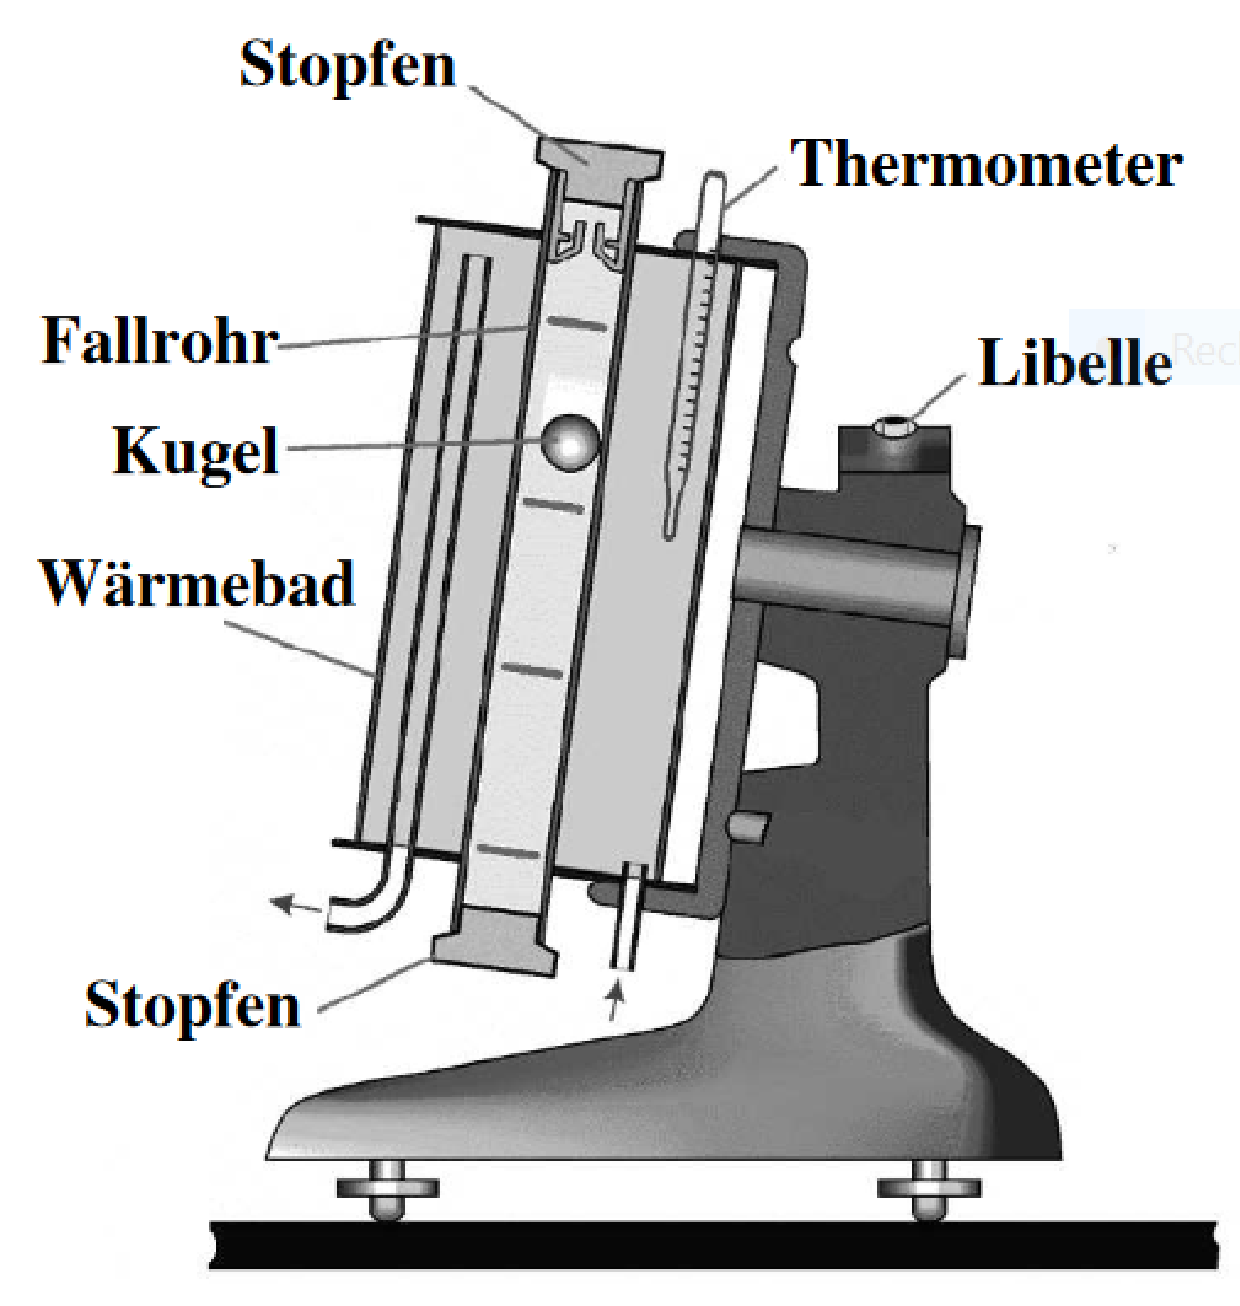
\includegraphics[width=5cm,height=10cm,keepaspectratio]{Viskosimeter.pdf} %Name und datityp von dem Bild (am besten geht PDF einfach in Adobe Acrobat unter Werkzeuge -> PDF erstellen -> und dann ein belibiges Bild auswählen der macht aus allem ne PDF und es wird sofort passend skaliert. Die PDF muss dann im Ordner Viskosimeter gespeichert sein nicht in content)
  \caption{Höppler-Viskosimeter} % Bildunterschrift
  \label{fig:vanadium}
\end{figure}
\subsection{Durchführung}
Zunächst wurde die Kugelkonstante der großen Kugel bestimmt. Dafür wurde sowohl für die große, als auch für die kleine Kugel jeweils zehn mal die Fallzeit bei Raumtemparatur bestimmt. Anschließend wurde für die Bestimmung der Temparaturabhängigkeit für 10 verschiedene Temparaturwerte zwischen $20.5°C$ und $88.9°C$ jeweils drei mal die Fallzeit der gr0ßen Kugel bestimmt.
